\documentclass{beamer}

%\usepackage{url}
\usepackage{listings}
\graphicspath{ {./img/} }

\title{Composite Pattern}
\author{Vladimir Martinka}
\institute{IBM}
\date{\today}

\begin{document}

\frame{\titlepage}

\section{Definition}
\begin{frame}{Definition}
	\begin{itemize}
	    \item Compose objects into tree structures to represent part-whole hierarchies. Composite lets clients treat individual objects and compositions of objects uniformly. \cite{gofComposite}
	\end{itemize}
\end{frame}

\begin{frame}{UML}
    \begin{figure}[h]
        \caption{Abstract structure of Composite pattern \cite{gofComposite}}
        \centering
        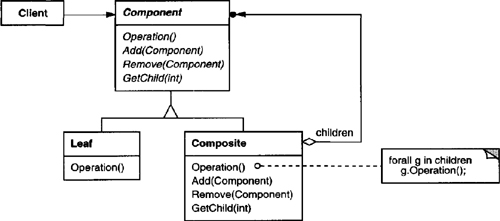
\includegraphics[width=\textwidth]{compositeUml}
    \end{figure}
\end{frame}

\begin{frame}{Example structure}
    \begin{figure}[h]
        \caption{Example composite object structure \cite{gofComposite}}
        \centering
        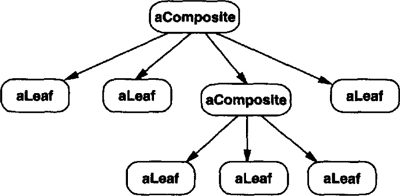
\includegraphics[width=\textwidth]{compositeExample}
    \end{figure}
\end{frame}

\section{Usage}
\begin{frame}{Usage}
    \begin{itemize}
        \item Graphics (parent draws subcomponents)
        \item Tree-structured reports
        \item Shopping cart
        \item \ldots
    \end{itemize}
\end{frame}

\section{Code example}
\begin{frame}[fragile]{Code example}{Component interface}
    \begin{lstlisting}[language=Java]
public interface CartItem {
    BigDecimal getPrice(); //operation
    
    void add(CartItem item);
    void remove(CartItem item);
    default List<CartItem> getChildren() {
        return Collections.emptyList();
    }
}
    \end{lstlisting}
\end{frame}

\begin{frame}{Code example}{Composite}
    \begin{figure}[h]
        \centering
        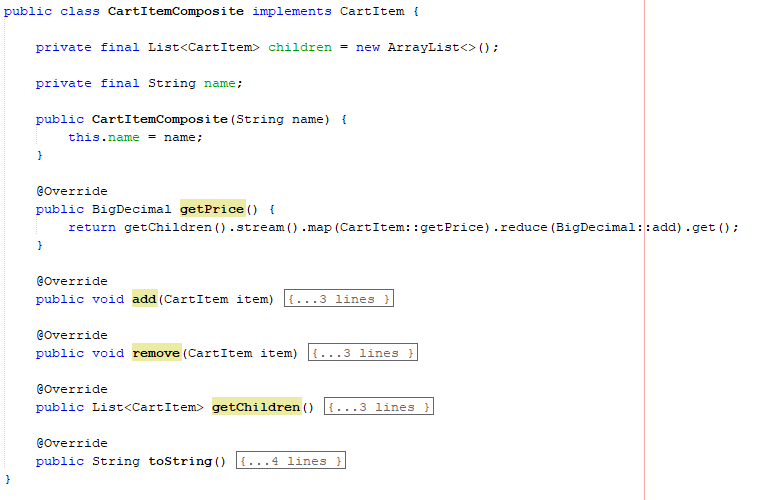
\includegraphics[width=\textwidth]{compositeCode}
    \end{figure}
\end{frame}

\begin{frame}{Code example}{Leaf}
    \begin{figure}[h]
        \centering
        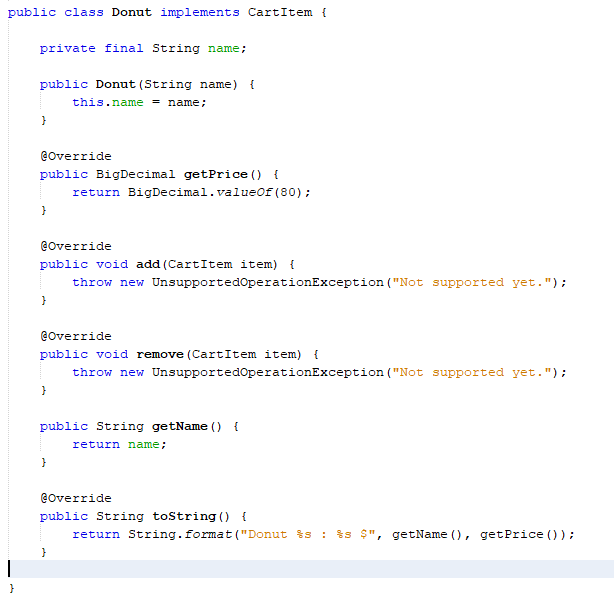
\includegraphics[width=\textwidth]{donutLeaf}
    \end{figure}
\end{frame}

\begin{frame}{Code example}{Client}
    \begin{figure}[h]
        \centering
        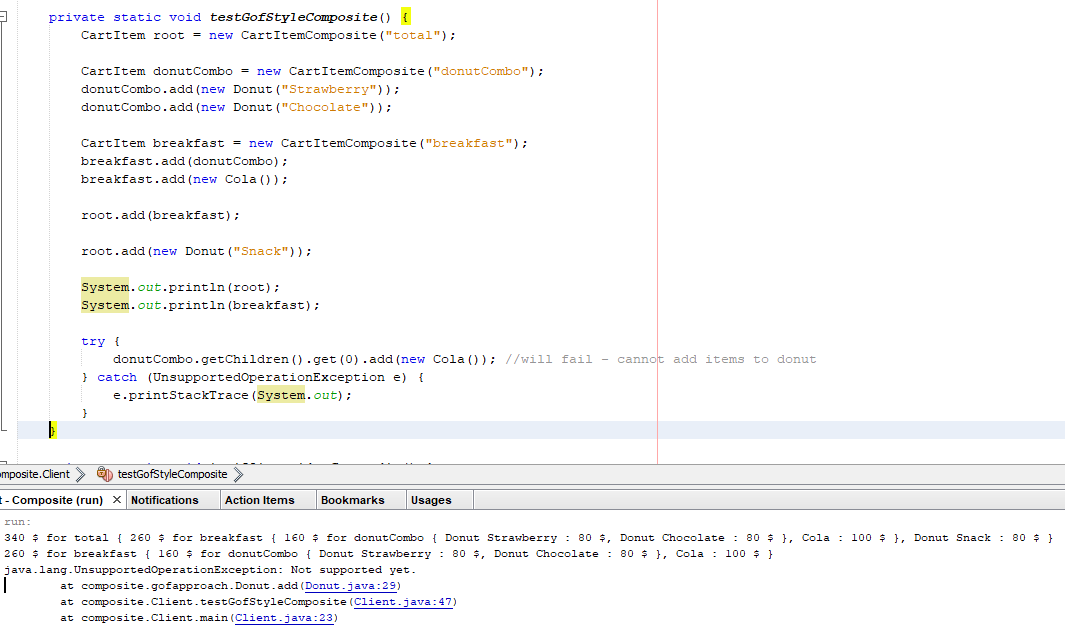
\includegraphics[width=\textwidth]{compositeTest}
    \end{figure}
\end{frame}


\section{Summary}
\begin{frame}{Summary}
\cite{gofComposite} Use the Composite pattern when 
\begin{itemize}
    \item you want to represent part-whole hierarchies of objects.
    \item you want clients to be able to ignore the difference between compositions of objects and individual objects. Clients will treat all objects in the composite structure uniformly.
\end{itemize}

Watch out for
\begin{itemize}
        \item Violation of single responsibility principle
        \item Design can get too general, client has no control over implementation, if that becomes necessary, run time checks may be required
        \item Children do not support all common operations - requires handling with some trade-offs in either safety or transparency
    \end{itemize}
\end{frame}

\section{References}
\begin{frame}[allowframebreaks]{References}
    \nocite{compositeSrc}
    \nocite{thisPresentation}
    

    \bibliographystyle{abbrv}
    \bibliography{references}
\end{frame}


\end{document}
